\chapter{Development}

\label{ch:conclusions}

\section{Introduction}

As explained in the design chapter, this project includes three deliverables. So the development will include; a Mac app dashboard, Perfect web-server and CocoaPods framework. Using the "tree-shaped" methodology the web-server was split up into their separate sections which include development, testing, and run. Then each service was design, developed and testing before moving up the tree. The development then broken up into phases, this way the project can be kept on track on what has been completed and whats left to do.

\begin{enumerate}
  \item Services Development
  \item Integrate into Live App
  \item Dashboard Development
  \item CocoaPod Framework 
\end{enumerate}

\section{Project Management}

Good software project management is essential in developing and delivery of software projects. Software development is often difficult to estimate the time required to complete the project, especially when using new technologies. Project milestones can be used to monitor the development progress of the project at certain key points. Above includes the list of the key points within the project. Each point had its own time frame; this kind of project can lead to expanding to including more services and tools, so sticking to the list will help be on schedule.

This project differs from commercial project, in that the project manager, designer, developer and tester were all the same person. And with any project, testing plays a major role in software development and can easily be left out. So self-discipline was required as there was no "boss" to answer to. 

\section{Services Development}

Each service had it's own Perfect server application along with Playground app. This made is easy to decide whether or not it was possible to implement each service into the project. For some of the services, the same Perfect web-server was used and able to be adapted to accommodate the requests needed. 

\paragraph{Setup} Before any development was started, some services was required to be setup. Perfect web-server developers provides an "assistant" to help with the setup and include and required packages needed to develop the API. The list of packages for the project include the following:

\begin{enumerate}
  \item https://github.com/PerfectlySoft/Perfect-Turnstile-MongoDB.git
  
  -Used to provide functionality to interact with MongoDB database, and provide authentication when requests come to the server.
  \item https://github.com/PerfectlySoft/Perfect-RequestLogger.git
  
  -Provides the web-server with a logging system.
  \item https://github.com/hkellaway/Gloss.git
  \item https://github.com/PerfectlySoft/Perfect-Notifications.git
  
  -Aid with the push notifications.
  \item https://github.com/PerfectlySoft/Perfect-SMTP.git
  
  -To be able to send Mails
  \item https://github.com/PerfectlySoft/Perfect-Zip.git
  
  -To zip backups folders, when sending to remote location.
\end{enumerate}

\newpage

After the Perfect web-server was setup, the mongoDB was required to installed locally. This was done by running the following commands in list \ref{lst:mongodb}

\lstinputlisting[label={lst:mongodb}, language=Bash, caption=MongoDB setup]{development/code/mongo.m}


\lstinputlisting[label={lst:playground},language=Swift, caption=Playgrounds setup]{development/code/playground.m}

To be able to run asynchronous code in the playgrounds, the following lines of code in list \ref{lst:playground} is required to be added to the top of the file. This will to make asynchronous code and get results.

\subsubsection{Database storage}

\paragraph{Design}
% A protocol was design to provide the following functionality that all structures conforming to 
TBJSONSerializable
As part of the project architecture with regarding to storage, any structure should have the functionality to send to the server, and retrieve without the need to create another function to setup and communication over HTTP. As described in the design chapter, all structures conforming to the protocol will be able to send and retrieve the object/s between the server and the application. JSON is used in the transfer of data, a format in which both server and client can understand. JSON objects are simply just dictionaries where each value has an object of some type.

To be able to parse each object to JSON, the object is first mirrored which is a representation of the sub-structure. This mirror is then looped over each property, depending on the type will depended on how it is parsed. When the loop has finished, the result is a dictionary which can be parsed into a string of JSON objects and sent to the server. The design also stated that in reprieving objects, functionality is to be in placed to parse back to objects. Using protocol extension to type alias of dictionary and method chaining, a list of functions was implemented to parse each value back to the desired type. The method chaining speeds the development time for the developer, without needing to find the correct result.  

\paragraph{Implementation}
The database storage required an object role model (ORM) which is a powerful method for designing and querying database models at the conceptual level, where the application is described in terms easily understood by non-technical database developers. It is a technique for converting data between incompatible type systems in object-oriented programming languages. The ORM was developed using Playground tool, where the creation of objects and parsing into JSON objects. The functionality of the ORM is to create a new object, parse it and send to the server, and be able to bring all objects back from the server. Extra functionality was added to be able to send filters.

\begin{figure}[!h]
    \caption{Storage Sequence Standard}
    \centering
    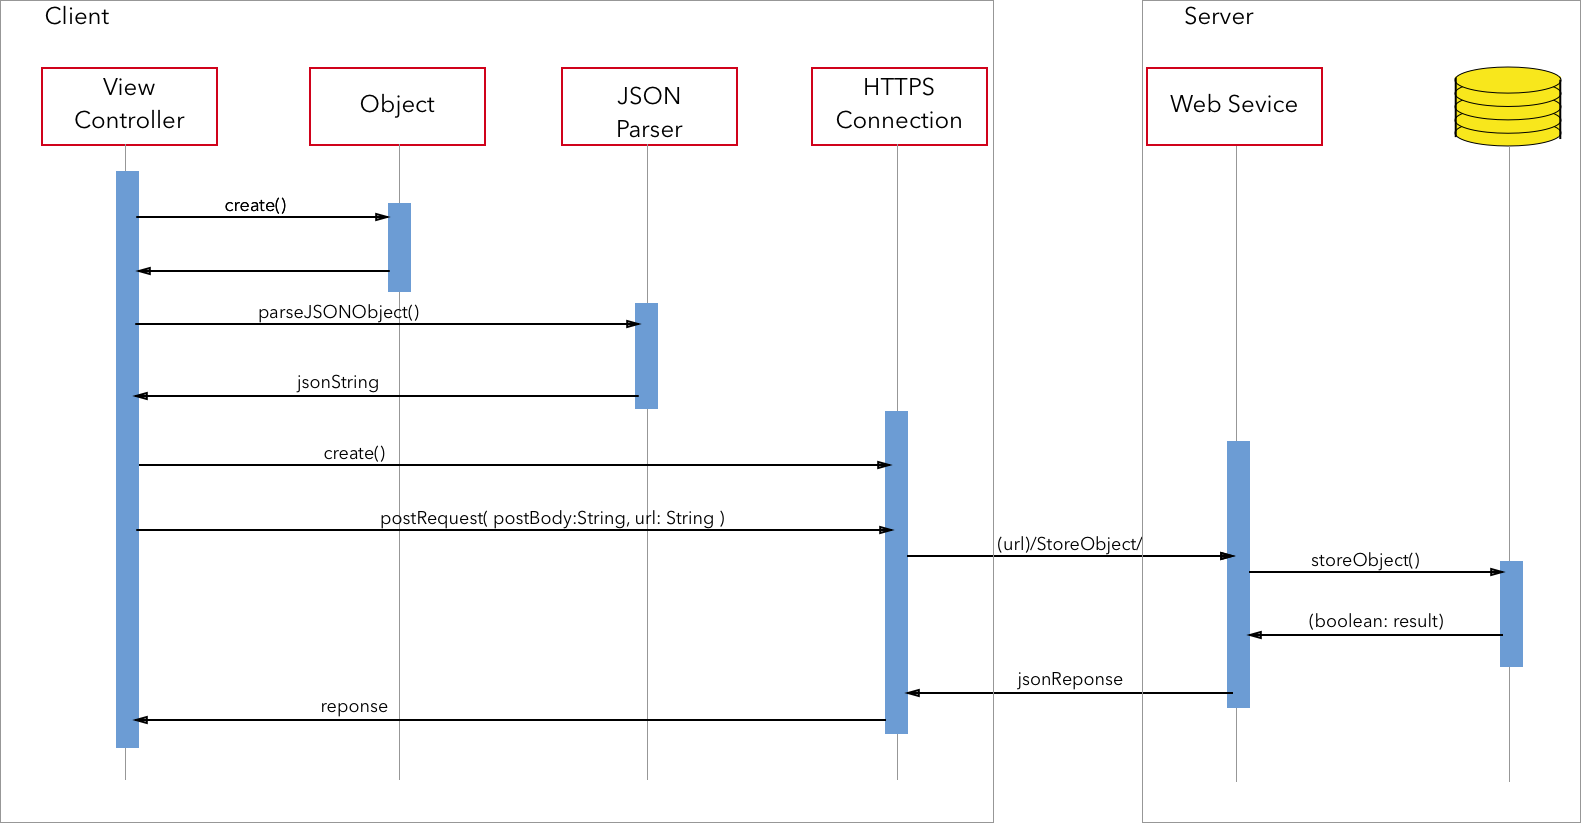
\includegraphics[width=100mm]{images/services/storage_sequence_current}
    \label{fig:storage_old}
\end{figure}


\begin{figure}[!h]
    \caption{Storage Sequence New}
    \centering
    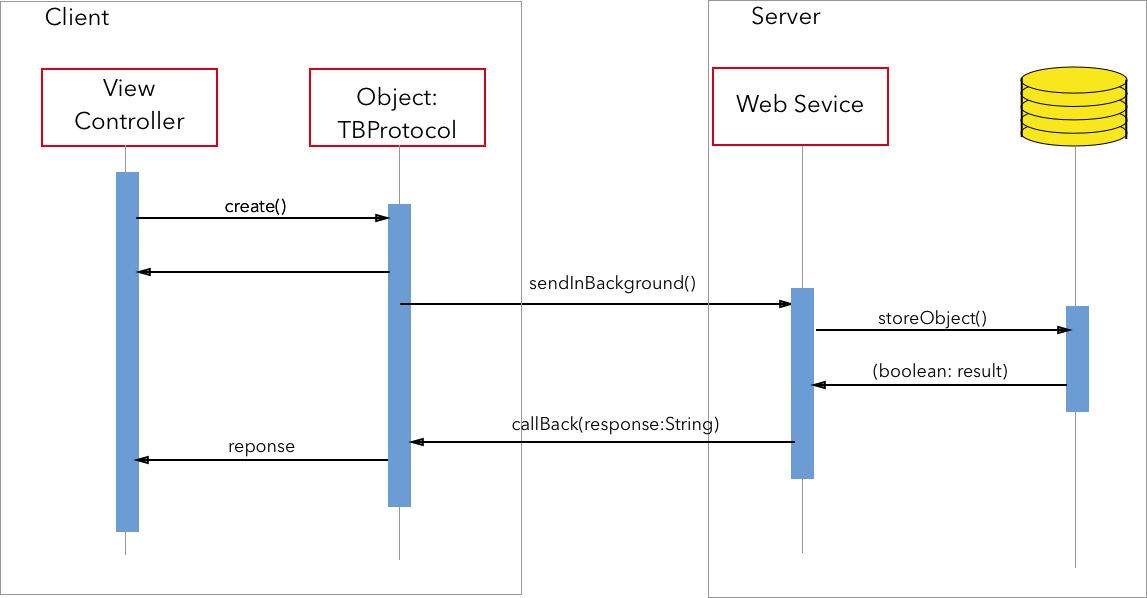
\includegraphics[width=100mm]{images/services/storage_sequence}
    \label{fig:storage_new}
\end{figure}

The two figures above show the difference to developing the standard way, with the developing having to create a JSON parser and then set-up a HTTPS connection to send it to the server in Fig \ref{fig:storage_old} . The new way in Fig \ref{fig:storage_new} using the project's storage protocol involves the developer only having to create the object, then using the objects functionality to send it to the server.

\subsubsection{Apple Push Notifications (APNs)}

\paragraph{Server}

Push notifications requires a number of steps to be implemented. First the .p8 key was downloaded, then the Perfect server test project required accessing that file to send notifications. Using the DIT-Timetable app to receive the push notifications.  

\begin{figure}[!h]
    \caption{APNs \cite{apns}}
    \centering
    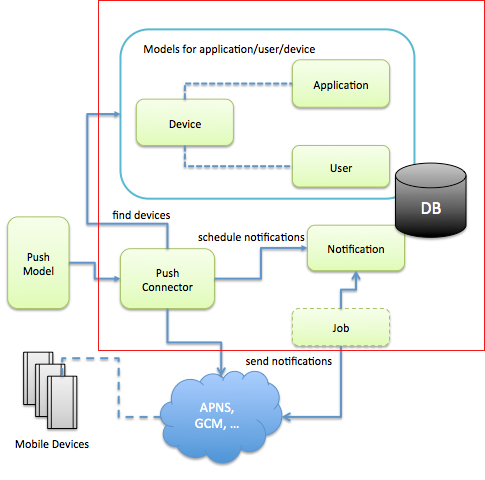
\includegraphics[width=75mm]{images/APNs}
    \label{fig:apns}
\end{figure}

In fig \ref{fig:apns} represents the stages in which to send push notifications. Inside the red box is the server layer, where the .p8 file is located, the push model is where the messages come from. The notifications goes through Apple's sandbox APNs, then on to the mobile devices.

\paragraph{Client}

APNs tool was implemented in the library, for which the developer can use the notification object to send request to the server, which in turn sends the notifications. The notifications object requires a list of values to be set for the notifications to work.

\begin{itemize}
  \item Universally Unique Identifiers
  - the targets device unique id to which apple will the notification
  \item Message
  - message which source wants to send to the target
  \item Badge Number
  - each notification can be assigned a number, which display on the app icon
  \item Title
  - the title of the notification, usually the app name
\end{itemize}

The following table \ref{table:mob_apns} demonstrates notification library to send notifications.

\begin{table}[!h]
\centering
\caption{APNS Library}
\label{table:mob_apns}
\begin{tabular}{|c|c|c|c|}
\hline
\rowcolor{green!20}
Library Method                    & Description                        & Parameters    & Result              \\ 
\hline
TBNotification.sendNotification();        & \makecell{Sends notifications\\ object to server} &  None & Successful/ Error   \\ 
\hline
\end{tabular}%
\end{table}

Fig \ref{table:apns} shows how to use the API requests outside of the library.

\begin{table}[!h]
\centering
\caption{Analytics API Requests}
\label{table:apns}
\begin{tabular}{|l|l|l|l|}
\hline
\rowcolor{green!20}
API Call                        & HTTP Method & Description                    & Parameters   \\ \hline
/\{appKey\}/notification & POST        & send notification object       & JSON Object  \\ \hline
/\{appKey\}/storage/TBNotification & GET         & Retrieves all notification objects & JSON Objects \\ \hline
\end{tabular}
\end{table}


\subsubsection{Analytics}

\paragraph{Level 1}

The first part for the analytic developed was the creation of the Perfect web-server which excepted POST requests. A playground application was developed with the lines of code in list \ref{lst:playground} to aid with HTTP requests. This class made gathers some information before sending the request, this include, time-stamp, build version, OS version, device make and model. For the purposes of testing this service, the data was hard-coded in separate function, that in turn would be reading from plist file. Some of methods and the parameters are included in the following table \ref{table:mob_analytics} shows how to use the library to send analytics. The server stores the analytic objects in the database corresponding to the application, this is done using the appKey which is sent up in the API request.

\begin{table}[!h]
\centering
\caption{Analytics Library}
\label{table:mob_analytics}
\begin{tabular}{|c|c|c|c|}
\hline
\rowcolor{green!20}
Library Method                    & Description                        & Parameters    & Result              \\ 
\hline
TBAnalytics.sendOpenApp();        & \makecell{Sends up object\\ with open app type} &   \makecell{view: UIView , \\ method: String? = \#function \\ , file: String? = \#file } & Successful/ Error   \\ 
\hline
TBAnayltics.send();               & \makecell{Send up object \\ with type as option} &  \makecell{ app: UIResponder, \\ type: SendType \\ , method: String? = \#function ,  \\ file: String? = \#file } & Successful/ Error   \\ 
\hline
 \makecell{ TBAnayltics \\.getAllInBackground(); } & \makecell{Retrieves all \\ TBAnayltic objects }   & NONE        & Array of TBAnayltics \\ 
\hline
\end{tabular}%
\end{table}

Fig \ref{table:analytics} shows how to use the API requests outside of the library.

\begin{table}[!h]
\centering
\caption{Analytics API Requests}
\label{table:analytics}
\begin{tabular}{|l|l|l|l|}
\hline
\rowcolor{green!20}
API Call                        & HTTP Method & Description                    & Parameters   \\ \hline
/\{appKey\}/storage/TBAnalytics & POST        & Uploads analytics object       & JSON Object  \\ \hline
/\{appKey\}/storage/TBAnalytics & GET         & Retrieves all analytic objects & JSON Objects \\ \hline
\end{tabular}
\end{table}


\subsubsection{Backup}


\subsubsection{Self hosted}


\subsubsection{Remote Configuration}

The remote configuration service development is broken up into four sections.

\begin{itemize}
  \item JSON files 
  - where the configuration objects will reside on the phone
  \item JSON file manager
  - how we will retrieve the values
  \item Objects configuration
  - how each interface object can be configured
  \item Remote change
  - will be discussed in the dashboard development
\end{itemize}

This section will discuss the first three, the remote change will be explained in dashboard development section.

\paragraph{JSON files}

The first part was the development of the JSON file layout. The design chapter already discussed the design of the remote configuration, where each class object will contain the objects relating to that class, and subsequently the objects properties will be in the object. To help with this, the storage protocol TBJSONSerializable was used to be able to parse the objects into JSON string. In listing \ref{lst:config} shows the base structure of the configuration object.

\lstinputlisting[label={lst:config},language=Swift, caption=Configuration Structure]{development/code/config.m}

In listing \ref{lst:config} lines 3 - 6 inclusive, holds the configuration objects for the applications. The colours objects is where all colours used in the app will be, this was placed here to speed up retrieval of each colour. The controllers objects is an array of view classes used within the app, then subsequently not shown are the objects within each class, and the properties relating to each object. The mainSettings variable on the same line of colours was placed here to speed up the retrieval of any import key values in the app such as URL. Last the languages list holds the list of languages available to the application. The languages part is based on the same as configuration files.

Lines 8 - 13 are to distinguishes this configuration file with another, so when an update of configuration is done, then the application call tell if it has the latest or needs to download. This is to stop re-downloading the same file over and over again. The following listing \ref{table:json_manager} shows the library methods which to use the remote configuration files.

\paragraph{JSON file manager}

\begin{table}[!h]
\centering
\caption{JSON file manager}
\label{table:json_manager}
\begin{tabular}{|c|c|c|c|}
\hline
\rowcolor{green!20}
Library Method                    & Description                        & Parameters    & Result              \\ 
\hline
RCConfigManager.getColor();        & \makecell{retrieval of\\ colour} &   \makecell{ name: String, defaultColor: UIColor } & UIColor   \\ 
\hline
 \makecell{RCConfigManager\\.getTranslation(); }  & \makecell{retrieval of\\ translation value} &  \makecell{  name: String, defaultName: String  } & String  \\ 
\hline
\makecell{ RCConfigManager \\.getMainSetting(); } & \makecell{retrieves main\\ setting value  }   & \makecell{  name: String, defaultName: String } & String \\ 
\makecell{ RCConfigManager \\.getObjectProperties(); } & \makecell{retrieves object\\ properties  }   & \makecell{  className: String, objectName: String } & [String:AnyObject] \\ 
\hline
\makecell{ RCConfigManager \\.getConfigVersion(); } & \makecell{gets latest version\\ of config file  }   & None & call back method \\ 
\hline
\makecell{ RCConfigManager \\.getConfigThemeVersion(); } & \makecell{gets latest version\\ of config theme file  }   & None & call back method \\ 
\hline
\end{tabular}
\end{table}


\paragraph{Objects configuration}

Object configurations involves how to get the object properties and update the user interface (UI) object. In the design chapter, it was discussed that a protocol along with protocol extension will be used on each UI object. A separate protocol for each UI object will be developed. To do this, a protocol is first define, then an extension on that protocol to add the implementation. A snippet example of UILabel UI Object is in the following listing \ref{lst:protocol}

The extension LabelLoad is restricted for classes with type UILabel, and the developer has two methods it can use to implement. Inside the setup first, the object properties is retrieved from the JSON files, and then set to the corresponding property value.

\lstinputlisting[label={lst:protocol},language=Swift, caption=UILabel Protocol]{development/code/protocol.m}

\subsubsection{A/B Testing}

A/B Testing utilizes two other services, remote configuration and Analytics. Using the JSON files, it can tell us what version of configuration is being used, so when an analytic object is sent up, then we include the version. The server however needs some development to handle A/B Testing. The dashboard explained later is used to set what applications, version of time the testing will be done. When a request comes into the web-server for configuration file, a check on the A/B Testing list is done to check whether that app version exists. 

To develop this service on the server, a singleton class "RemoteConfig" is used. When the server starts up, the singleton class is initialized with a current request number of zero. With each request, the count increases, and using this value can depend on what version of the configuration file that users gets.

\subsubsection{Live Database}


\subsubsection{Exception catching}

The design chapter explained there are two types of exception catching, uncaught and caught exceptions. Both types need to developed in different ways, as one would potentially crash the app, so not able to send POST request to the server. Not only are there two types of exceptions, but each exception has a different level, so when the developer views the dashboard, they can set a priority. The different levels are Fatal, Error, Warning, Info and Debug.

The exception was developed using a singleton class to that all exceptions can be sent through. When the app opens, the exception objects gets initialised which includes setting the NSSetUncaughtExceptionHandler(), where the parameter is an internal function name which looks after catching the exception. The values that will be sent up to server include the following:

\begin{itemize}
  \item time-stamp
  \item build version
  \item OS version
  \item device make and model
  \item exception name
  \item exception reason
  \item user info if any
  \item stack trace
  \item stack symbols
\end{itemize}

\paragraph{Uncaught exceptions}
Uncaught exceptions makes the app crashes, so between the time crash happens and the app closes which is a small window, the exception has to be dealt with. Using the NSSetUncaughtExceptionHandler() with the parameter of function, that function is not allowed to make outside calls, which include HTTP request and function calls. So the exception is stored in UserDefaults which is a built in data dictionary that stores small amount of user settings for as long as the app is stored. When the user opens application again, the exception singleton class gets instantiated, and it does a check if any exceptions exists in UserDefaults, and then a HTTP post sends the exception to the server.

\paragraph{Caught exceptions}


\section{Integrate into Live App}

For some parts of project, an already developed and published app called DIT-Timetable was used to add in the services, to test if Apple would allow it through. The services include remote configuration and language choice. Due to Apple's strict guidelines, the remote configuration was developed into the DIT-Timetable app into two stages, then each stage had a build and published.

\subsubsection{Phase 1}
This phase included just the basic remote configuration, with the capability of updating text such as page title, and label values. Apple did approve this phase, and while the app live, using the iPad prototyping app the text values were able to be changed. 

\subsubsection{Phase 2}

Phase 2 gave the ability to adjust user interface values such as text colour, text size and user interaction enabling/disabling. This also been approved by Apple giving it a go ahead to be completely integrated into the project.  

\section{Dashboard Development}

The dashboard was originally going to be created as an iPad app, but after some thought that not all mobile developers can be expected to own an iPad, the dashboard was developed as a Mac App. In the design chapter, the layout and design of the dashboard was discussed including what functionality will be provided to the developers.

\section{CocoaPod Framework}

The CocoaPod was left to last to development, as all the test cases used in the Playground could be brought over and adjusted to fit the framework. After the CocoaPod was finished, a test project was created for external professional mobile developers to use and give some feedback.